\chapter{总体设计}
%==================================================================
\section{软件描述}
    系统包括前台和后台两个部分。
\subsection{前台主要功能}
    向服务器发送请求,并接受服务器的响应,向用户展示服务器的返回结果。
    
    \begin{itemize}
        \item 用户可以进行账户注册,并使用已经注册的账户登录该系统。
        \item 用户可以与其他用户进行聊天。除了基本的文字聊天,用户还可以进行音视频聊天。此外,用户可以查看自己的聊天记录。
        \item 用户可以在群聊中发言。如果身份是管理员或群主,用户还可以对群聊进行管理。此外,不同的群聊情境还会提供不同的额外群聊功能。
        \item 用户可以对自己的通讯录进行管理:可以添加或删除好友,在添加好友时系统会进行个性化推荐;可以加入或退出群聊;可以将其他用户移入或移出黑名单。
        \item 用户可以对自己的Board进行管理,新建或修改日志;也可以浏览他人的Board,对他们的日志进行评论。
        \item 用户可以进行在线文档协作。
        \item 在接收到新的信息时,用户可以得到提醒。
        \item 用户在加入组织后,可以进行活动管理,自动修改所有参与者的日历。
        \item 用户可以查看并修改自己的日历。  
        \item 用户可以管理本地和云端的文件。
        \item 用户可以将账号与邮箱或设备进行绑定,以提高账户的安全性。
        \item 用户可以通过邮箱接口得知是否有新的邮件。
    \end{itemize}
    
\subsection{后台主要功能}
后台服务器接收用户发送的动作和请求,予以处理并进行响应。

服务器在接收到用户请求时,会在服务器的数据库中进行查询操作,并且进
行返回查询结果或者反馈提示信息,对于用户提交的数据(比如发布活动、修改日志等),也会存入到数据库中。对于发送的聊天信息,服务器会将其缓存到发送队列中。

%==================================================================
\section{处理流程}
    %--------------------------------------------------------------
    \subsection{总体流程}
        此处应当有一个图和对应的描述。
        \begin{figure}[ht]
            \centering
            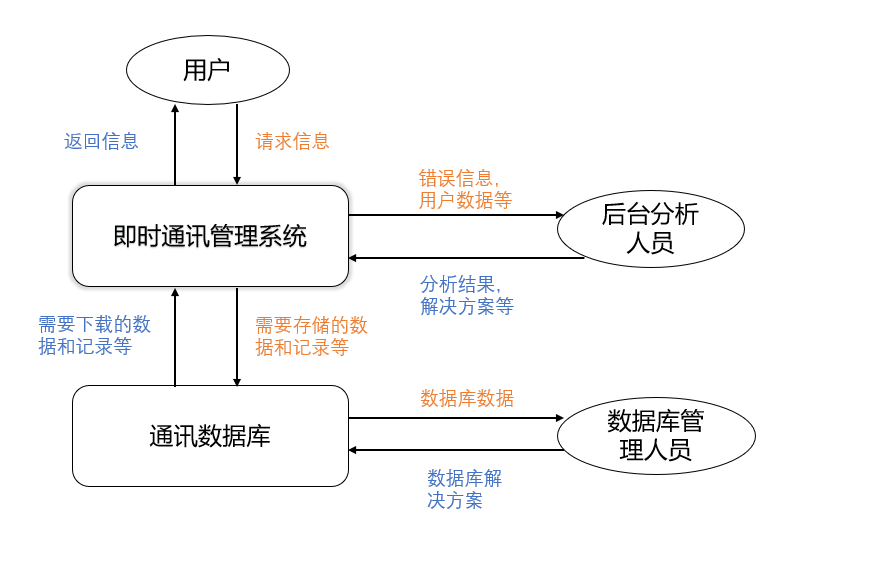
\includegraphics[scale = 0.75]{总体流程.png}\label{tab:classification}
            \caption{总体流程}\label{fig:noted-figure}
        \end{figure}
    %--------------------------------------------------------------
    \subsection{系统基本流程}
        此处应当有一个图和对应的描述。
    %--------------------------------------------------------------
    \subsection{客户端基本流程}
        这只是举个例子,如果没有客户端则不需要此节。
    %--------------------------------------------------------------
    \subsection{服务器端基本流程}
    服务器端流程如图\ref{fig:server_flow}所示。客户端1和2展示了一对一聊天和群聊的服务器处理过程;客户端4和5展示了音视频通讯的过程;
    客户端1与服务器间的箭头展示了查询的过程;客户端3与服务器间的箭头展示了更新的过程(许多功能都可以抽象为查询和更新,在后面会详细说明)。
    服务器使用SQL语句向数据库集群发送查询或更新请求,集群返回查询或更新的结果。
        \begin{figure}
            \centering
            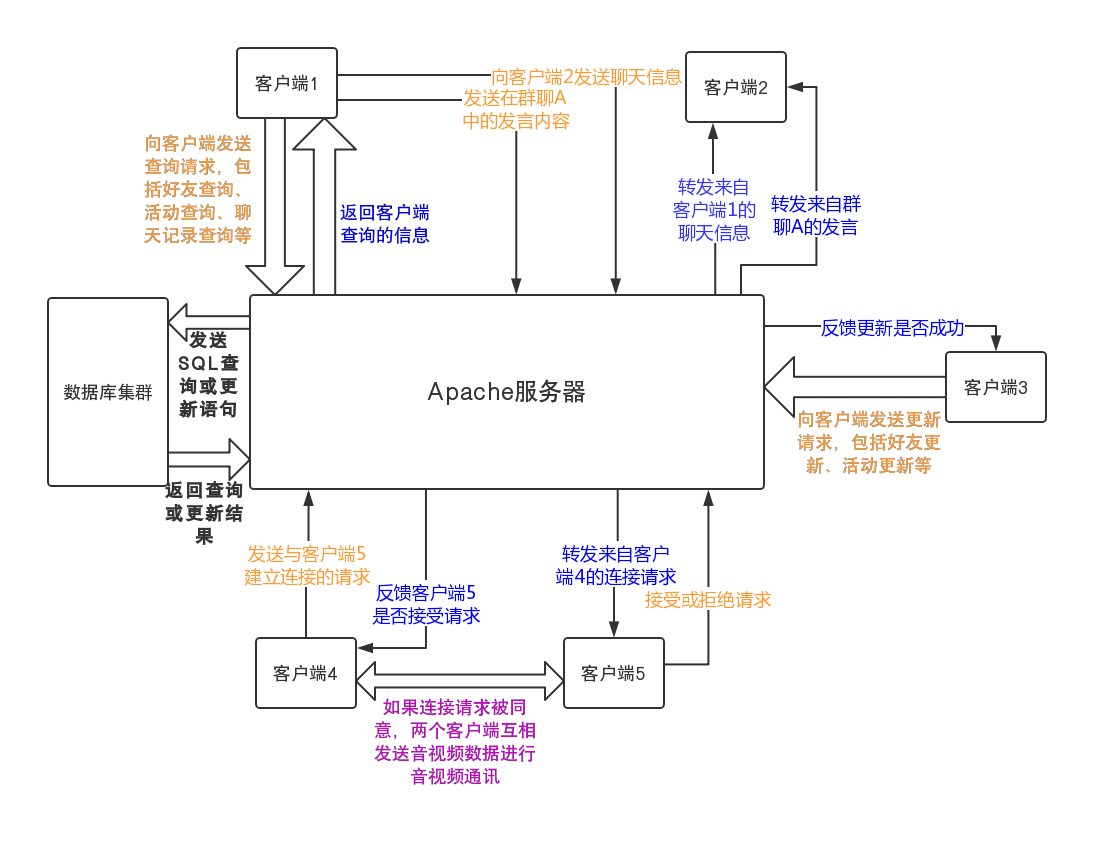
\includegraphics[scale=0.4]{OutlineDesign/figures/server_flow.png}
            \caption{服务器端流程}
            \label{fig:server_flow}
        \end{figure}
    %--------------------------------------------------------------
    \subsection{R.INTF.CALC.001: 一对一即时通讯功能·具体流程}
        已登录用户
    %--------------------------------------------------------------
%================ EXAMPLE ===================================================
% 已登录用户在购物车中提交请求交易的 POST 请求,提交的表单中指明了交易中包括的
% 所有商品、商家、付款信息、收货地址,输入输出处理系统接收到合法请求后,向商品信息
% 系统请求数据,收到数据以后验证是否正确,然后向订单系统发起生成新订单的请求,订单
% 系统负责更新商品信息系统、商家信息,通知商家接单,返回订单处理结果输入输出处理系
% 统,输入输出处理系统依照结果产生 HTML 页面,并返回给用户。
%================ EXAMPLE ===================================================
    \subsection{R.INTF.CALC.002: 多情境群聊功能·具体流程}
        %--------------------------------------------------------------
        \subsubsection{R.INTF.CALC.002.1: 群管理·具体流程}
        %--------------------------------------------------------------
        \subsubsection{R.INTF.CALC.002.2: 群聊天·具体流程}
        %--------------------------------------------------------------
        \subsubsection{R.INTF.CALC.002.3: 情境功能·具体流程}
        %--------------------------------------------------------------
    \subsection{R.INTF.CALC.003: 活动/任务发布与管理功能·具体流程}
    %--------------------------------------------------------------
    \subsection{R.INTF.CALC.004: 音视频通话 (会议) 功能·具体流程}
    %--------------------------------------------------------------
    \subsection{R.INTF.CALC.005: 通讯录功能·具体流程}
        %--------------------------------------------------------------
        \subsubsection{R.INTF.CALC.005.1: 好友管理·具体流程}
        %--------------------------------------------------------------
        \subsubsection{R.INTF.CALC.005.2: 群聊管理·具体流程}
        %--------------------------------------------------------------
        \subsubsection{R.INTF.CALC.005.3: 黑名单·具体流程}
        %--------------------------------------------------------------
    \subsection{R.INTF.CALC.006: 聊天记录功能·具体流程}
    %--------------------------------------------------------------
    \subsection{R.INTF.CALC.007: 消息提醒功能·具体流程}
    %--------------------------------------------------------------
    \subsection{R.INTF.CALC.008: Board(广场) 功能·具体流程}
    %--------------------------------------------------------------
    \subsection{R.INTF.CALC.009: 个性化好友推荐功能·具体流程}
    %--------------------------------------------------------------
    \subsection{R.INTF.CALC.010: 在线文档协作平台功能·具体流程}
    %--------------------------------------------------------------
    \subsection{R.INTF.CALC.011: 账号保护和隐私保护功能·具体流程}
    %--------------------------------------------------------------
    \subsection{R.INTF.CALC.012: 日历管理功能·具体流程}
    %--------------------------------------------------------------
    \subsection{R.INTF.CALC.013: 个人本地和云端文件管理功能·具体流程}
    %--------------------------------------------------------------
    \subsection{R.INTF.CALC.014: 邮箱接口功能·具体流程}
    %--------------------------------------------------------------
%==================================================================
\section{功能结构设计}
    %--------------------------------------------------------------
    \subsection{整体结构}
    
%============================== GUIDE ========================================
% 此处应当有一个图和对应的描述。系统如果像微内核那样,划分成核心模块和若干个子
% 系统,此处应当有图示及说明,然后后续几个节应当描述这几个子系统。如果系统像宏
% 内核,那应当说明有哪些紧密联系的模块,并在后续几个节内描述这些模块。
%============================== GUIDE ========================================
    \subsection{用户端结构}
%============================== GUIDE ========================================
% 此处应当有一个图和对应的描述。这只是举个例子。可能的内容包括用户端的具体模
% 块、耦合情况等。
%============================== GUIDE ========================================
    \subsection{服务器端结构}
%============================== GUIDE ========================================
% 此处应当有一个图和对应的描述。这只是举个例子。
%============================== GUIDE ========================================
    \subsection{后台数据库维护模块结构}
%============================== GUIDE ========================================
% 此处应当有一个图和对应的描述。这只是举个例子。
%============================== GUIDE ========================================
%==================================================================
\section{功能需求与程序代码的关系}
%============================== GUIDE ========================================
% [此处指的是不同的需求分配到哪些模块去实现。可按不同的端拆分此表]
%============================== GUIDE ========================================
    \begin{table}[htbp]
        \centering
        \small
        \caption{功能需求与程序代码的关系表} \label{tab:requirement-module}
            \begin{tabular}{|p{9em}|p{2.5em}|p{2.5em}|p{2.5em}|p{2.5em}|p{2.5em}|
                            p{2.5em}|p{2.5em}|p{2.5em}|}
            \hline %**********************************************************
            ·   & 用户信息管理模块      & 错误信息处理模块  & 云文件管理模块 
                & 文件管理模块          & 日历管理模块      & 团队管理模块      
                & 在线文档协作平台模块  & 通讯管理模块\\
            \hline %**********************************************************
            R.INTF.CALC.001: 一对一即时通讯功能
            %   & 用户信息管理模块      & 错误信息处理模块  & 云文件管理模块 
                & Y                     & Y                 & · 
            %   & 文件管理模块          & 日历管理模块      & 团队管理模块  
                & Y                     & ·                 & · 
            %   & 在线文档协作平台模块  & 通讯管理模块      \\
                & ·                     & Y                 \\
            \hline  %**********************************************************
            R.INTF.CALC.002: 多情境群聊功能
            %   & 用户信息管理模块      & 错误信息处理模块  & 云文件管理模块 
                & Y                     & Y                 & Y
            %   & 文件管理模块          & 日历管理模块      & 团队管理模块  
                & Y                     & ·                 & Y 
            %   & 在线文档协作平台模块  & 通讯管理模块      \\
                & ·                     & Y                 \\
            \hline %**********************************************************
            R.INTF.CALC.003: 活动/任务发布与管理功能
            %   & 用户信息管理模块      & 错误信息处理模块  & 云文件管理模块 
                & Y                     & Y                 & · 
            %   & 文件管理模块          & 日历管理模块      & 团队管理模块  
                & ·                     & Y                 & Y 
            %   & 在线文档协作平台模块  & 通讯管理模块      \\
                & ·                     & ·                 \\
            \hline %**********************************************************
            R.INTF.CALC.004: 音视频通话 (会议) 功能
            %   & 用户信息管理模块      & 错误信息处理模块  & 云文件管理模块 
                & Y                     & Y                 & · 
            %   & 文件管理模块          & 日历管理模块      & 团队管理模块  
                & ·                     & ·                 & · 
            %   & 在线文档协作平台模块  & 通讯管理模块      \\
                & ·                     & Y                 \\
            \hline %**********************************************************
            R.INTF.CALC.005: 通讯录功能
            %   & 用户信息管理模块      & 错误信息处理模块  & 云文件管理模块 
                & Y                     & Y                 & · 
            %   & 文件管理模块          & 日历管理模块      & 团队管理模块  
                & ·                     & ·                 & · 
            %   & 在线文档协作平台模块  & 通讯管理模块      \\
                & ·                     & ·                 \\
            \hline %**********************************************************
            R.INTF.CALC.006: 聊天记录功能
            %   & 用户信息管理模块      & 错误信息处理模块  & 云文件管理模块 
                & Y                     & Y                 & · 
            %   & 文件管理模块          & 日历管理模块      & 团队管理模块  
                & ·                     & ·                 & · 
            %   & 在线文档协作平台模块  & 通讯管理模块      \\
                & ·                     & Y                 \\
            \hline %**********************************************************
            R.INTF.CALC.007: 消息提醒功能
            %   & 用户信息管理模块      & 错误信息处理模块  & 云文件管理模块 
                & Y                     & Y                 & · 
            %   & 文件管理模块          & 日历管理模块      & 团队管理模块  
                & ·                     & Y                 & Y 
            %   & 在线文档协作平台模块  & 通讯管理模块      \\
                & ·                     & Y                 \\
            \hline %**********************************************************
            R.INTF.CALC.008: Board(广场)功能
            %   & 用户信息管理模块      & 错误信息处理模块  & 云文件管理模块 
                & Y                     & Y                 & · 
            %   & 文件管理模块          & 日历管理模块      & 团队管理模块  
                & ·                     & Y                 & · 
            %   & 在线文档协作平台模块  & 通讯管理模块      \\
                & ·                     & ·                 \\
            \hline %**********************************************************
            R.INTF.CALC.009: 个性化好友推荐功能
            %   & 用户信息管理模块      & 错误信息处理模块  & 云文件管理模块 
                & Y                     & Y                 & · 
            %   & 文件管理模块          & 日历管理模块      & 团队管理模块  
                & ·                     & ·                 & · 
            %   & 在线文档协作平台模块  & 通讯管理模块      \\
                & ·                     & Y                 \\
            \hline %**********************************************************
            R.INTF.CALC.010: 在线文档协作平台功能
            %   & 用户信息管理模块      & 错误信息处理模块  & 云文件管理模块 
                & Y                     & Y                 & Y 
            %   & 文件管理模块          & 日历管理模块      & 团队管理模块  
                & ·                     & ·                 & Y 
            %   & 在线文档协作平台模块  & 通讯管理模块      \\
                & Y                     & ·                 \\
            \hline %**********************************************************
            R.INTF.CALC.011: 账号保护和隐私保护功能
            %   & 用户信息管理模块      & 错误信息处理模块  & 云文件管理模块 
                & Y                     & Y                 & · 
            %   & 文件管理模块          & 日历管理模块      & 团队管理模块  
                & ·                     & ·                 & · 
            %   & 在线文档协作平台模块  & 通讯管理模块      \\
                & ·                     & ·                 \\
            \hline %**********************************************************
            R.INTF.CALC.012: 日历管理功能
            %   & 用户信息管理模块      & 错误信息处理模块  & 云文件管理模块 
                & Y                     & Y                 & · 
            %   & 文件管理模块          & 日历管理模块      & 团队管理模块  
                & ·                     & Y                 & Y 
            %   & 在线文档协作平台模块  & 通讯管理模块      \\
                & ·                     & ·                 \\
            \hline %**********************************************************
            R.INTF.CALC.013: 个人本地和云端文件管理功能
            %   & 用户信息管理模块      & 错误信息处理模块  & 云文件管理模块 
                & Y                     & Y                 & Y 
            %   & 文件管理模块          & 日历管理模块      & 团队管理模块  
                & Y                     & ·                 & · 
            %   & 在线文档协作平台模块  & 通讯管理模块      \\
                & Y                     & Y                 \\
            \hline %**********************************************************
            R.INTF.CALC.014: 邮箱接口功能
            %   & 用户信息管理模块      & 错误信息处理模块  & 云文件管理模块 
                & Y                     & Y                 & · 
            %   & 文件管理模块          & 日历管理模块      & 团队管理模块  
                & ·                     & ·                 & · 
            %   & 在线文档协作平台模块  & 通讯管理模块      \\
                & ·                     & ·                 \\
            \hline %**********************************************************
            \end{tabular}
        \note{本表体现了各项功能需求的实现与各个程序模块的分配关系}
    \end{table}
%==================================================================